\chapter{Ағындар мен қималар}

Бұл тарауда төмендегі екі есепті 
қарастыратын боламыз:

\begin{itemize}
\item \key{Максималды ағынды табу}, яғни 
бір төбеден екінші төбеге максималды қанша 
ағын жібере алатынымызды анықтау.
\item \key{Минималды қиманы табу}, яғни
графта салмағы минималды болатын
қай қырлар жиындысы 
екі төбенің арасын ажырататынын анықтау.
\end{itemize}

Аталған екі есепте де бағытталған,
салмақталған граф пен
екі арнаулы төбе берілген. Мұндағы
\emph{бастау} -- кіріс қырлары жоқ төбе,
\emph{саға} –– шығыс қырлары жоқ төбе.

Өрнек ретінде бастауы 1-төбе,
ал сағасы 6-төбе болатын төмендегі графты қолданамыз:

\begin{center}
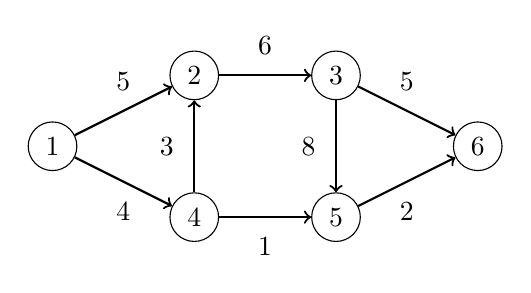
\begin{tikzpicture}[scale=0.9]
\node[draw, circle] (1) at (1,2) {$1$};
\node[draw, circle] (2) at (3,3) {$2$};
\node[draw, circle] (3) at (5,3) {$3$};
\node[draw, circle] (4) at (7,2) {$6$};
\node[draw, circle] (5) at (3,1) {$4$};
\node[draw, circle] (6) at (5,1) {$5$};
\path[draw,thick,->] (1) -- node[font=\small,label=5] {} (2);
\path[draw,thick,->] (2) -- node[font=\small,label=6] {} (3);
\path[draw,thick,->] (3) -- node[font=\small,label=5] {} (4);
\path[draw,thick,->] (1) -- node[font=\small,label=below:4] {} (5);
\path[draw,thick,->] (5) -- node[font=\small,label=below:1] {} (6);
\path[draw,thick,->] (6) -- node[font=\small,label=below:2] {} (4);
\path[draw,thick,<-] (2) -- node[font=\small,label=left:3] {} (5);
\path[draw,thick,->] (3) -- node[font=\small,label=left:8] {} (6);
\end{tikzpicture}
\end{center}

\subsubsection{Максималды ағын}

\index{ағын}
\index{Максималды ағын}

Ең \key{максималды ағын} есебіндегі
бізге берілетін тапсырама -- бастаудан сағаға
ең максималды ағынды жіберу. Әр қырдағы салмақ --
сол қыр арқылы қанша ағын өте алатынын шектеуші
сыйымдылық. Әр аралық төбенің кіріс және шығыс
ағындары бірдей болуы қажет. 

Өрнектегі графтың максималды ағыны -- 7.
Ал төмендегі сурет ағынды қалай бағыттау
керектігін көрсетеді:

\begin{center}
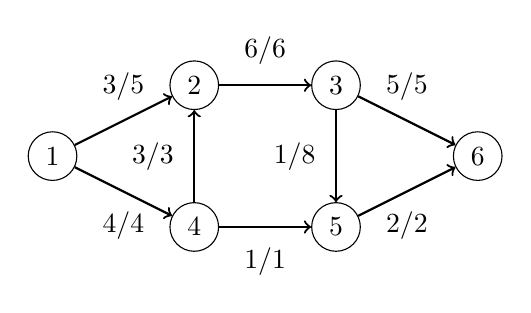
\begin{tikzpicture}[scale=0.9]
\node[draw, circle] (1) at (1,2) {$1$};
\node[draw, circle] (2) at (3,3) {$2$};
\node[draw, circle] (3) at (5,3) {$3$};
\node[draw, circle] (4) at (7,2) {$6$};
\node[draw, circle] (5) at (3,1) {$4$};
\node[draw, circle] (6) at (5,1) {$5$};
\path[draw,thick,->] (1) -- node[font=\small,label=3/5] {} (2);
\path[draw,thick,->] (2) -- node[font=\small,label=6/6] {} (3);
\path[draw,thick,->] (3) -- node[font=\small,label=5/5] {} (4);
\path[draw,thick,->] (1) -- node[font=\small,label=below:4/4] {} (5);
\path[draw,thick,->] (5) -- node[font=\small,label=below:1/1] {} (6);
\path[draw,thick,->] (6) -- node[font=\small,label=below:2/2] {} (4);
\path[draw,thick,<-] (2) -- node[font=\small,label=left:3/3] {} (5);
\path[draw,thick,->] (3) -- node[font=\small,label=left:1/8] {} (6);
\end{tikzpicture}
\end{center}

$v/k$ нотациясы -- $k$ бірлік сыйымдылығы бар
қырдан $v$ бірлік ағын бағытталғанын көрсетеді.  
Ағынның өлшемі -- $7$, себебі бастау $3+4$ бірлік 
ағын жіберіп, саға $5+2$ ағынды қабылдайды. 
Бұл жағдайда ағын максималды екенін түсіну 
оңай, өйткені сағаға жетелейтін барлық 
қырлардың сыйымдылығы -- 7.

\subsubsection{Минималды қима}

\index{қима}
\index{минималды қима}

\key{Минималды қима} есебіндегі
бізге берілетін тапсырма графта 
бастаудан сағаға жол болмайтындай етіп
қырлар жиындысын өшіруге және өшірілген 
қырлардың салмағы минималды болуына арналады. 

Өрнек графындағы қиманың минималды өлшемі -- 7.
$2 \rightarrow 3$ пен $4 \rightarrow 5$ қырларын
өшіру жеткілікті:

\begin{center}
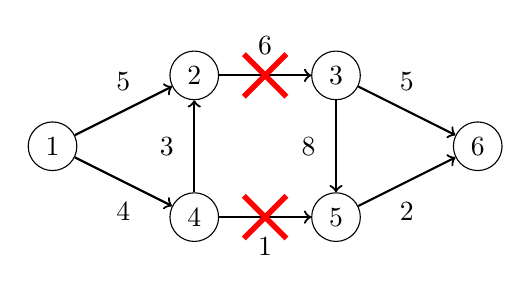
\begin{tikzpicture}[scale=0.9]
\node[draw, circle] (1) at (1,2) {$1$};
\node[draw, circle] (2) at (3,3) {$2$};
\node[draw, circle] (3) at (5,3) {$3$};
\node[draw, circle] (4) at (7,2) {$6$};
\node[draw, circle] (5) at (3,1) {$4$};
\node[draw, circle] (6) at (5,1) {$5$};
\path[draw,thick,->] (1) -- node[font=\small,label=5] {} (2);
\path[draw,thick,->] (2) -- node[font=\small,label=6] {} (3);
\path[draw,thick,->] (3) -- node[font=\small,label=5] {} (4);
\path[draw,thick,->] (1) -- node[font=\small,label=below:4] {} (5);
\path[draw,thick,->] (5) -- node[font=\small,label=below:1] {} (6);
\path[draw,thick,->] (6) -- node[font=\small,label=below:2] {} (4);
\path[draw,thick,<-] (2) -- node[font=\small,label=left:3] {} (5);
\path[draw,thick,->] (3) -- node[font=\small,label=left:8] {} (6);

\path[draw=red,thick,-,line width=2pt] (4-.3,3-.3) -- (4+.3,3+.3);
\path[draw=red,thick,-,line width=2pt] (4-.3,3+.3) -- (4+.3,3-.3);
\path[draw=red,thick,-,line width=2pt] (4-.3,1-.3) -- (4+.3,1+.3);
\path[draw=red,thick,-,line width=2pt] (4-.3,1+.3) -- (4+.3,1-.3);
\end{tikzpicture}
\end{center}

Қырларды өшіргеннен кейін бастаудан сағаға дейін
ешқандай жол болмайды. Қиманың өлшемі -- 7, ал өшірілген
қырлардың салмақтары -- $6$ мен $1$. Жалпы салмағы $7$-ден кем болатын өшіруге келетін қырлар жиындысы
графта болмағандықтан қима минималды деп саналады.
\\\\
Жоғарыдағы өрнекте максималды ағын 
мен минималды қиманың 
бірдей болуы жай сәйкестік емес. 
Шын мәнінде олар \emph{әрқашан} тең болады. 
Сондықтан бұл ұғымдар 
әртүрлі болып көрінгенімен, өте тығыз байланысты.

Алдағы уақытта біз максималды ағын мен
минималды қиманы табатын Форд-Фалкерсон 
алгоритмін талқылайтын боламыз. Алгоритм
олардың \emph{не} себепті тең екенін түсінуімізге 
көмектеседі. 

\section{Форд–Фалкерсон алгоритмі}

\index{Форд–Фалкерсон алгоритмі}

\key{Форд–Фалкерсон алгоритмі} \cite{for56} 
графтағы максималды ағынды табады. Алгоритм
бос ағыннан басталады, әр қадамда бастаудан 
сағаға дейін көбірек ағын өндіретін жолды іздейді.
Ақырында алгоритм ағынды үлкейте алмаса, 
максималды ағын табылады. 

Алгоритм әр негізгі қырға 
оған кері бағытта қыр болатын графтың арнайы көрінісін қолданады.
Әр қырдың салмағы тағы қанша ағынның өте алатынын 
бейнелейді. Алгоритмнің басында негізгі қырлардың
салмақтары сол қырлардың сыйымдылықтарына тең болса,
кері қырлардың салмақтары нөлге тең болады.


\begin{samepage}
Өрнек графының жаңа көрінісі төмендегідей болады:

\begin{center}
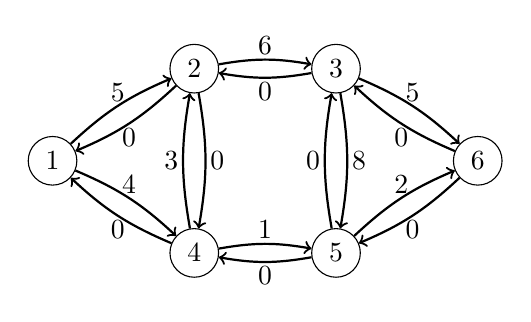
\begin{tikzpicture}[scale=0.9,label distance=-2mm]
\node[draw, circle] (1) at (1,1.3) {$1$};
\node[draw, circle] (2) at (3,2.6) {$2$};
\node[draw, circle] (3) at (5,2.6) {$3$};
\node[draw, circle] (4) at (7,1.3) {$6$};
\node[draw, circle] (5) at (3,0) {$4$};
\node[draw, circle] (6) at (5,0) {$5$};

\path[draw,thick,->] (1) edge [bend left=10] node[font=\small,label=5] {} (2);
\path[draw,thick,->] (2) edge [bend left=10] node[font=\small,label=below:0] {} (1);
\path[draw,thick,->] (2) edge [bend left=10] node[font=\small,label=6] {} (3);
\path[draw,thick,->] (3) edge [bend left=10] node[font=\small,label=below:0] {} (2);
\path[draw,thick,->] (3) edge [bend left=10] node[font=\small,label=5] {} (4);
\path[draw,thick,->] (4) edge [bend left=10] node[font=\small,label=below:0] {} (3);
\path[draw,thick,->] (1) edge [bend left=10] node[font=\small,label=4] {} (5);
\path[draw,thick,->] (5) edge [bend left=10] node[font=\small,label=below:0] {} (1);
\path[draw,thick,->] (5) edge [bend left=10] node[font=\small,label=1] {} (6);
\path[draw,thick,->] (6) edge [bend left=10] node[font=\small,label=below:0] {} (5);
\path[draw,thick,->] (6) edge [bend left=10] node[font=\small,label=2] {} (4);
\path[draw,thick,->] (4) edge [bend left=10] node[font=\small,label=below:0] {} (6);
\path[draw,thick,->] (5) edge [bend left=10] node[font=\small,label=left:3] {} (2);
\path[draw,thick,->] (2) edge [bend left=10] node[font=\small,label=right:0] {} (5);
\path[draw,thick,->] (3) edge [bend left=10] node[font=\small,label=right:8] {} (6);
\path[draw,thick,->] (6) edge [bend left=10] node[font=\small,label=left:0] {} (3);
\end{tikzpicture}
\end{center}
\end{samepage}

\subsubsection{Алгоритм сипаттамасы}

Форд-Фалкерсон алгоритмі бірнеше кезеңдерден
тұрады. Әр кезеңде алгоритм барлық қырлардың салмақтары
оң болатын бастаудан сағаға жол іздейді.
Егер мұндай бірнеше жол болса, кез келгенін 
таңдай аламыз. 

Мысалы, төмендегідей жолды таңдайық:

\begin{center}
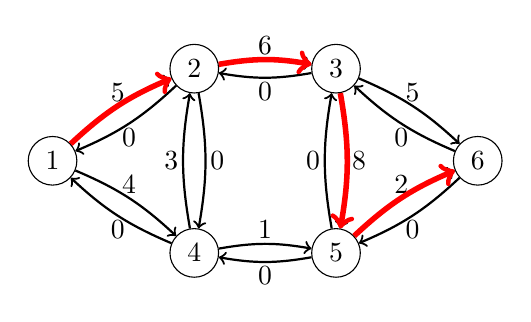
\begin{tikzpicture}[scale=0.9,label distance=-2mm]
\node[draw, circle] (1) at (1,1.3) {$1$};
\node[draw, circle] (2) at (3,2.6) {$2$};
\node[draw, circle] (3) at (5,2.6) {$3$};
\node[draw, circle] (4) at (7,1.3) {$6$};
\node[draw, circle] (5) at (3,0) {$4$};
\node[draw, circle] (6) at (5,0) {$5$};

\path[draw,thick,->] (1) edge [bend left=10] node[font=\small,label=5] {} (2);
\path[draw,thick,->] (2) edge [bend left=10] node[font=\small,label=below:0] {} (1);
\path[draw,thick,->] (2) edge [bend left=10] node[font=\small,label=6] {} (3);
\path[draw,thick,->] (3) edge [bend left=10] node[font=\small,label=below:0] {} (2);
\path[draw,thick,->] (3) edge [bend left=10] node[font=\small,label=5] {} (4);
\path[draw,thick,->] (4) edge [bend left=10] node[font=\small,label=below:0] {} (3);
\path[draw,thick,->] (1) edge [bend left=10] node[font=\small,label=4] {} (5);
\path[draw,thick,->] (5) edge [bend left=10] node[font=\small,label=below:0] {} (1);
\path[draw,thick,->] (5) edge [bend left=10] node[font=\small,label=1] {} (6);
\path[draw,thick,->] (6) edge [bend left=10] node[font=\small,label=below:0] {} (5);
\path[draw,thick,->] (6) edge [bend left=10] node[font=\small,label=2] {} (4);
\path[draw,thick,->] (4) edge [bend left=10] node[font=\small,label=below:0] {} (6);
\path[draw,thick,->] (5) edge [bend left=10] node[font=\small,label=left:3] {} (2);
\path[draw,thick,->] (2) edge [bend left=10] node[font=\small,label=right:0] {} (5);
\path[draw,thick,->] (3) edge [bend left=10] node[font=\small,label=right:8] {} (6);
\path[draw,thick,->] (6) edge [bend left=10] node[font=\small,label=left:0] {} (3);

\path[draw=red,thick,->,line width=2pt] (1) edge [bend left=10] (2);
\path[draw=red,thick,->,line width=2pt] (2) edge [bend left=10] (3);
\path[draw=red,thick,->,line width=2pt] (3) edge [bend left=10] (6);
\path[draw=red,thick,->,line width=2pt] (6) edge [bend left=10] (4);
\end{tikzpicture}
\end{center}

Жолды таңдағаннан кейін ағын $x$ бірлікке артады,
мұнда $x$ -- жолдағы ең кіші салмақ. Оған қоса
жолдағы қырлардың салмақтарын $x$-ке азайтамыз және
кері қырлардың салмақтарын $x$-ке арттырамыз.  

Жоғарыдағы жолда қырлардың салмақтары
-- 5, 6, 8 және 2. Ең кіші салмақ -- 2, 
жаңа граф төмендегідей:

\begin{center}
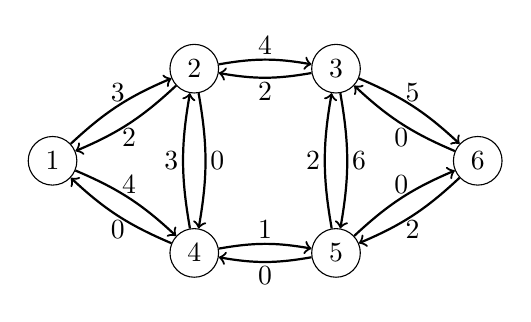
\begin{tikzpicture}[scale=0.9,label distance=-2mm]
\node[draw, circle] (1) at (1,1.3) {$1$};
\node[draw, circle] (2) at (3,2.6) {$2$};
\node[draw, circle] (3) at (5,2.6) {$3$};
\node[draw, circle] (4) at (7,1.3) {$6$};
\node[draw, circle] (5) at (3,0) {$4$};
\node[draw, circle] (6) at (5,0) {$5$};

\path[draw,thick,->] (1) edge [bend left=10] node[font=\small,label=3] {} (2);
\path[draw,thick,->] (2) edge [bend left=10] node[font=\small,label=below:2] {} (1);
\path[draw,thick,->] (2) edge [bend left=10] node[font=\small,label=4] {} (3);
\path[draw,thick,->] (3) edge [bend left=10] node[font=\small,label=below:2] {} (2);
\path[draw,thick,->] (3) edge [bend left=10] node[font=\small,label=5] {} (4);
\path[draw,thick,->] (4) edge [bend left=10] node[font=\small,label=below:0] {} (3);
\path[draw,thick,->] (1) edge [bend left=10] node[font=\small,label=4] {} (5);
\path[draw,thick,->] (5) edge [bend left=10] node[font=\small,label=below:0] {} (1);
\path[draw,thick,->] (5) edge [bend left=10] node[font=\small,label=1] {} (6);
\path[draw,thick,->] (6) edge [bend left=10] node[font=\small,label=below:0] {} (5);
\path[draw,thick,->] (6) edge [bend left=10] node[font=\small,label=0] {} (4);
\path[draw,thick,->] (4) edge [bend left=10] node[font=\small,label=below:2] {} (6);
\path[draw,thick,->] (5) edge [bend left=10] node[font=\small,label=left:3] {} (2);
\path[draw,thick,->] (2) edge [bend left=10] node[font=\small,label=right:0] {} (5);
\path[draw,thick,->] (3) edge [bend left=10] node[font=\small,label=right:6] {} (6);
\path[draw,thick,->] (6) edge [bend left=10] node[font=\small,label=left:2] {} (3);
\end{tikzpicture}
\end{center}

Идеясы ағынды арттыру арқылы болашақта қырлардан
өте алатын ағынды азайтуға бағытталады. Екінші жағынан
егер ағынды басқа жолмен өткізген оңтайлырақ болса,
өткізген ағынды графтағы кері қырлар арқылы болдырмауға болады.

Алгоритм бастаудан сағаға қырлардың
салмақтары оң болатын 
жол болғанша ағынды арттырады. Мысалдағы
келесі жолымыз төмендегідей болады:

\begin{center}
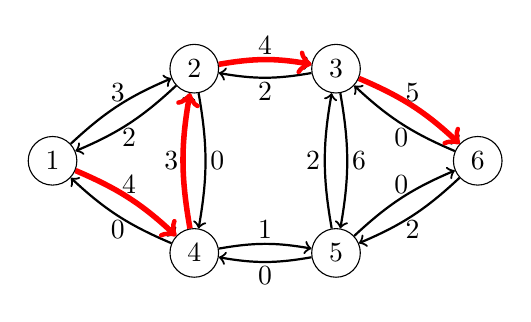
\begin{tikzpicture}[scale=0.9,label distance=-2mm]
\node[draw, circle] (1) at (1,1.3) {$1$};
\node[draw, circle] (2) at (3,2.6) {$2$};
\node[draw, circle] (3) at (5,2.6) {$3$};
\node[draw, circle] (4) at (7,1.3) {$6$};
\node[draw, circle] (5) at (3,0) {$4$};
\node[draw, circle] (6) at (5,0) {$5$};

\path[draw,thick,->] (1) edge [bend left=10] node[font=\small,label=3] {} (2);
\path[draw,thick,->] (2) edge [bend left=10] node[font=\small,label=below:2] {} (1);
\path[draw,thick,->] (2) edge [bend left=10] node[font=\small,label=4] {} (3);
\path[draw,thick,->] (3) edge [bend left=10] node[font=\small,label=below:2] {} (2);
\path[draw,thick,->] (3) edge [bend left=10] node[font=\small,label=5] {} (4);
\path[draw,thick,->] (4) edge [bend left=10] node[font=\small,label=below:0] {} (3);
\path[draw,thick,->] (1) edge [bend left=10] node[font=\small,label=4] {} (5);
\path[draw,thick,->] (5) edge [bend left=10] node[font=\small,label=below:0] {} (1);
\path[draw,thick,->] (5) edge [bend left=10] node[font=\small,label=1] {} (6);
\path[draw,thick,->] (6) edge [bend left=10] node[font=\small,label=below:0] {} (5);
\path[draw,thick,->] (6) edge [bend left=10] node[font=\small,label=0] {} (4);
\path[draw,thick,->] (4) edge [bend left=10] node[font=\small,label=below:2] {} (6);
\path[draw,thick,->] (5) edge [bend left=10] node[font=\small,label=left:3] {} (2);
\path[draw,thick,->] (2) edge [bend left=10] node[font=\small,label=right:0] {} (5);
\path[draw,thick,->] (3) edge [bend left=10] node[font=\small,label=right:6] {} (6);
\path[draw,thick,->] (6) edge [bend left=10] node[font=\small,label=left:2] {} (3);

\path[draw=red,thick,->,line width=2pt] (1) edge [bend left=10] (5);
\path[draw=red,thick,->,line width=2pt] (5) edge [bend left=10] (2);
\path[draw=red,thick,->,line width=2pt] (2) edge [bend left=10] (3);
\path[draw=red,thick,->,line width=2pt] (3) edge [bend left=10] (4);
\end{tikzpicture}
\end{center}

Осы жолдағы ең кіші қырдың салмағы -- 3,
демек жол ағынды 3-ке арттырады және осы жолды
өңдегеннен кейін қорытынды ағын 5 болады. 

\begin{samepage}
Жаңа граф төмендегідей:

\begin{center}
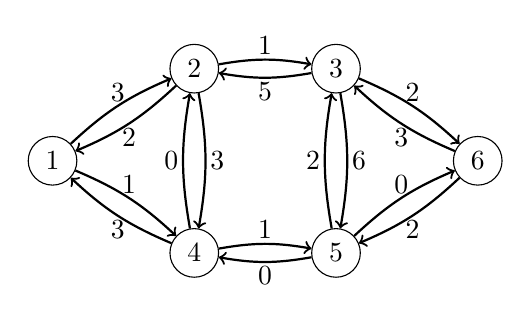
\begin{tikzpicture}[scale=0.9,label distance=-2mm]
\node[draw, circle] (1) at (1,1.3) {$1$};
\node[draw, circle] (2) at (3,2.6) {$2$};
\node[draw, circle] (3) at (5,2.6) {$3$};
\node[draw, circle] (4) at (7,1.3) {$6$};
\node[draw, circle] (5) at (3,0) {$4$};
\node[draw, circle] (6) at (5,0) {$5$};

\path[draw,thick,->] (1) edge [bend left=10] node[font=\small,label=3] {} (2);
\path[draw,thick,->] (2) edge [bend left=10] node[font=\small,label=below:2] {} (1);
\path[draw,thick,->] (2) edge [bend left=10] node[font=\small,label=1] {} (3);
\path[draw,thick,->] (3) edge [bend left=10] node[font=\small,label=below:5] {} (2);
\path[draw,thick,->] (3) edge [bend left=10] node[font=\small,label=2] {} (4);
\path[draw,thick,->] (4) edge [bend left=10] node[font=\small,label=below:3] {} (3);
\path[draw,thick,->] (1) edge [bend left=10] node[font=\small,label=1] {} (5);
\path[draw,thick,->] (5) edge [bend left=10] node[font=\small,label=below:3] {} (1);
\path[draw,thick,->] (5) edge [bend left=10] node[font=\small,label=1] {} (6);
\path[draw,thick,->] (6) edge [bend left=10] node[font=\small,label=below:0] {} (5);
\path[draw,thick,->] (6) edge [bend left=10] node[font=\small,label=0] {} (4);
\path[draw,thick,->] (4) edge [bend left=10] node[font=\small,label=below:2] {} (6);
\path[draw,thick,->] (5) edge [bend left=10] node[font=\small,label=left:0] {} (2);
\path[draw,thick,->] (2) edge [bend left=10] node[font=\small,label=right:3] {} (5);
\path[draw,thick,->] (3) edge [bend left=10] node[font=\small,label=right:6] {} (6);
\path[draw,thick,->] (6) edge [bend left=10] node[font=\small,label=left:2] {} (3);
\end{tikzpicture}
\end{center}
\end{samepage}

Максималды ағынға жетуіміз үшін 
әлі де 2 кезең өтуіміз қажет. 
Мысалы, біз $1 \rightarrow 2 \rightarrow 3 \rightarrow 6$
және 
$1 \rightarrow 4 \rightarrow 5 \rightarrow 3 \rightarrow 6$ жолдарын
таңдай аламыз. 
Екеуі де ағынды 1-ге арттырады және 
қорытынды граф төмендегідей болады:

\begin{center}
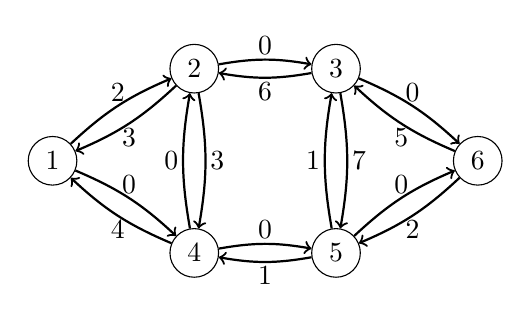
\begin{tikzpicture}[scale=0.9,label distance=-2mm]
\node[draw, circle] (1) at (1,1.3) {$1$};
\node[draw, circle] (2) at (3,2.6) {$2$};
\node[draw, circle] (3) at (5,2.6) {$3$};
\node[draw, circle] (4) at (7,1.3) {$6$};
\node[draw, circle] (5) at (3,0) {$4$};
\node[draw, circle] (6) at (5,0) {$5$};

\path[draw,thick,->] (1) edge [bend left=10] node[font=\small,label=2] {} (2);
\path[draw,thick,->] (2) edge [bend left=10] node[font=\small,label=below:3] {} (1);
\path[draw,thick,->] (2) edge [bend left=10] node[font=\small,label=0] {} (3);
\path[draw,thick,->] (3) edge [bend left=10] node[font=\small,label=below:6] {} (2);
\path[draw,thick,->] (3) edge [bend left=10] node[font=\small,label=0] {} (4);
\path[draw,thick,->] (4) edge [bend left=10] node[font=\small,label=below:5] {} (3);
\path[draw,thick,->] (1) edge [bend left=10] node[font=\small,label=0] {} (5);
\path[draw,thick,->] (5) edge [bend left=10] node[font=\small,label=below:4] {} (1);
\path[draw,thick,->] (5) edge [bend left=10] node[font=\small,label=0] {} (6);
\path[draw,thick,->] (6) edge [bend left=10] node[font=\small,label=below:1] {} (5);
\path[draw,thick,->] (6) edge [bend left=10] node[font=\small,label=0] {} (4);
\path[draw,thick,->] (4) edge [bend left=10] node[font=\small,label=below:2] {} (6);
\path[draw,thick,->] (5) edge [bend left=10] node[font=\small,label=left:0] {} (2);
\path[draw,thick,->] (2) edge [bend left=10] node[font=\small,label=right:3] {} (5);
\path[draw,thick,->] (3) edge [bend left=10] node[font=\small,label=right:7] {} (6);
\path[draw,thick,->] (6) edge [bend left=10] node[font=\small,label=left:1] {} (3);
\end{tikzpicture}
\end{center}

Бұдан кейін ағынды арттыру мүмкін емес, өйткені
бастаудан сағаға дейінгі қырлардың салмағы оң
болатын жол жоқ. 
Демек алгоритм тоқтайды және максималды ағын 7-ге тең болады.

\subsubsection{Жолдар іздеу}

Форд-Фалкерсон алгоритмі ағынды арттыратын қандай
жолдарды алу керектігін атап өтпейді. Кез келген
жағдайда алгоритм ерте ме, кеш пе, бір тоқтайды және 
максималды ағынды дұрыс табады. Бірақ алгоритмнің
тиімділігі жолдардың қалай таңдалғанына тәуелді болады.

Жолдарды табудың қарапайым тәсілі -- 
тереңдігі бойынша ізденісті (DFS) қолдану.
Әдетте бұл жақсы жұмыс істейді, бірақ ең нашар жағдайда
әр жол ағынды 1-ге арттыратындықтан, мұндай алгоритм
баяу өтеді. Бақытымызға орай, төмендегі әдістердің 
бірін қолдану арқылы бұл жағдайдан құтыла аламыз:

\index{Эдмондс-Карп алгоритмі}

\key{Эдмондс–Карп алгоритмі} \cite{edm72}
жолдағы қырлардың саны ең аз болатын
жолды таңдап отырады. Мұны тереңдігі бойынша ізденістің
(DFS) орнына ені бойынша ізденіс (BFS) жасау арқылы орындауымызға
болады. Сол арқылы ағынның жылдам өсу кепілдігін 
дәлелдей аламыз және алгоритмнің уақытша күрделілігі 
$O(m^2 n)$ болмақ.

\index{ағынды масштабтау алгоритмі}

\key{Ағынды масштабтау алгоритмі} \cite{ahu91} 
тереңдігі бойынша ізденіс (DFS) арқылы
жолдағы қырлардың салмағы кем дегенде шекті 
мән болатын жолдарды іздейді. Бастапқыда
шекті мән үлкен сан, мысалы
барлық қырлардың салмақтар қосындысы болуы мүмкін.
Жол табылмаған жағдайда шекті мәнді әрдайым
2-ге бөлеміз. Алгоритмнің уақытша күрделілігі ––
$O(m^2 \log c)$, мұндағы $c$ -- бастапқы шекті мән. 

Тәжірибеде ағынды масштабтау алгоритмін жазу жеңілірек, яғни 
жолдарды табу үшін тереңдігі бойынша ізденісті (DFS) қолдансақ жеткілікті.
Екі алгоритм де әдетте 
бағдарламалау контесттерінде
кездесетін есептер үшін 
жеткілікті деңгейде тиімді болады.

\subsubsection{Минималды қима}

\index{минималды қима}

Форд–Фалкерсон алгоритмі максималды ағынды тапқаннан кейін, 
минималды қиманы да анықтайды. 
$A$ деп бастаудан салмақтары оң қырлар арқылы
жетуге болатын төбелер жиындысын белгілейік. 
Өрнектегі графта $A$ 1, 2, және 4 төбелерінен тұрады:

\begin{center}
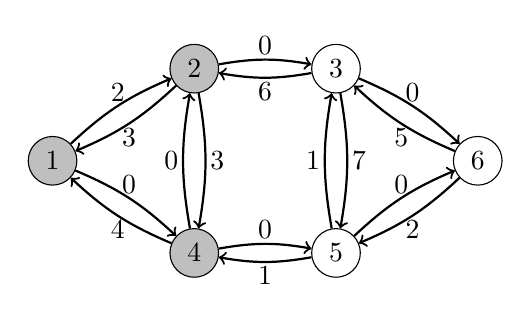
\begin{tikzpicture}[scale=0.9,label distance=-2mm]
\node[draw, circle,fill=lightgray] (1) at (1,1.3) {$1$};
\node[draw, circle,fill=lightgray] (2) at (3,2.6) {$2$};
\node[draw, circle] (3) at (5,2.6) {$3$};
\node[draw, circle] (4) at (7,1.3) {$6$};
\node[draw, circle,fill=lightgray] (5) at (3,0) {$4$};
\node[draw, circle] (6) at (5,0) {$5$};

\path[draw,thick,->] (1) edge [bend left=10] node[font=\small,label=2] {} (2);
\path[draw,thick,->] (2) edge [bend left=10] node[font=\small,label=below:3] {} (1);
\path[draw,thick,->] (2) edge [bend left=10] node[font=\small,label=0] {} (3);
\path[draw,thick,->] (3) edge [bend left=10] node[font=\small,label=below:6] {} (2);
\path[draw,thick,->] (3) edge [bend left=10] node[font=\small,label=0] {} (4);
\path[draw,thick,->] (4) edge [bend left=10] node[font=\small,label=below:5] {} (3);
\path[draw,thick,->] (1) edge [bend left=10] node[font=\small,label=0] {} (5);
\path[draw,thick,->] (5) edge [bend left=10] node[font=\small,label=below:4] {} (1);
\path[draw,thick,->] (5) edge [bend left=10] node[font=\small,label=0] {} (6);
\path[draw,thick,->] (6) edge [bend left=10] node[font=\small,label=below:1] {} (5);
\path[draw,thick,->] (6) edge [bend left=10] node[font=\small,label=0] {} (4);
\path[draw,thick,->] (4) edge [bend left=10] node[font=\small,label=below:2] {} (6);
\path[draw,thick,->] (5) edge [bend left=10] node[font=\small,label=left:0] {} (2);
\path[draw,thick,->] (2) edge [bend left=10] node[font=\small,label=right:3] {} (5);
\path[draw,thick,->] (3) edge [bend left=10] node[font=\small,label=right:7] {} (6);
\path[draw,thick,->] (6) edge [bend left=10] node[font=\small,label=left:1] {} (3);
\end{tikzpicture}
\end{center}

Енді минималды қима $A$-дағы төбеден басталып, $A$-ның сыртындағы төбеде
аяқталатын және максималды ағында сыйымдылығы толық қолданылған қырлардан 
тұрады. Жоғарыдағы графта сондай қырлар -- $2 \rightarrow 3$ 
және $4 \rightarrow 5$, олар $6+1=7$ минималды қимасын береді. 

''Неге алгоритмнен құрылған ағын максималды және
қима минималды болады?'' - деген сұрақ туындауы мүмкін. Оған мынадай түсіндірме береміз: графта
кез келген қиманың салмағынан үлкен
ағын болуы мүмкін емес. Демек ағын мен қиманың мәндері 
тең болса, онда ағын максималды, ал қима минималды болмақ.

Бастау $A$-да, саға $B$-да болатын
және екі жиынның араларында қырлары 
бар қималарды қарастырайық:

% Let us consider any cut of the graph
% such that the source belongs to $A$,
% the sink belongs to $B$
% and there are some edges between the sets:

\begin{center}
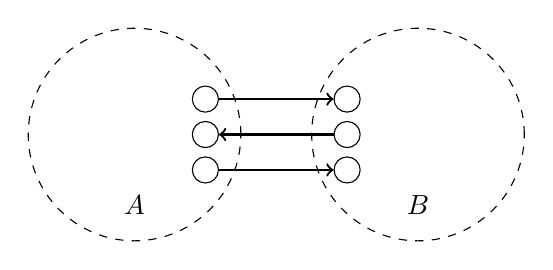
\begin{tikzpicture}[scale=0.9]
\draw[dashed] (-2,0) circle (1.5);
\draw[dashed] (2,0) circle (1.5);

\node at (-2,-1) {$A$};
\node at (2,-1) {$B$};

\node[draw, circle] (1) at (-1,0.5) {};
\node[draw, circle] (2) at (-1,0) {};
\node[draw, circle] (3) at (-1,-0.5) {};
\node[draw, circle] (4) at (1,0.5) {};
\node[draw, circle] (5) at (1,0) {};
\node[draw, circle] (6) at (1,-0.5) {};

\path[draw,thick,->] (1) -- (4);
\path[draw,thick,->] (5) -- (2);
\path[draw,thick,->] (3) -- (6);

\end{tikzpicture}
\end{center}

Қиманың өлшемі -- $A$ мен $B$ араларынан өтетін
қырлардың қосындысы. Бұл графтағы ағынның жоғарғы шекті 
мәні, себебі ағын $A$ мен $B$ арасынан өтуі қажет. 
Осылайша максималды ағынның өлшемі 
кез келген қиманың өлшемінен
кіші немесе тең болады.

Басқа жағынан қарасақ, Форд-Фалкерсон алгоритмі 
бір қиманың өлшеміне \emph{тең} ағынды табады. 
Осылайша ағын максималды және
қима минималды болуы керек. 

% On the other hand, the Ford–Fulkerson algorithm
% produces a flow whose size is \emph{exactly} as large
% as the size of a cut in the graph.
% Thus, the flow has to be a maximum flow
% and the cut has to be a minimum cut.

\section{Қиылыспайтын жолдар}

Граф есептерінің көбісін максималды ағын есебіне
келтіріп шығаруымызға болады. Сондай есептердің 
біріне мысал келтірейік. Бізге бастау мен сағасы бар 
бағытталған граф берілген. Тапсырма бойынша бастаудан сағаға апаратын
қиылыспайтын жолдардың максималды санын 
есептеуіміз керек. 

% Many graph problems can be solved by reducing
% them to the maximum flow problem.
% Our first example of such a problem is
% as follows: we are given a directed graph
% with a source and a sink,
% and our task is to find the maximum number
% of disjoint paths from the source to the sink.

\subsubsection{Қырлары қиылыспайтын жолдар}

Алдымен бастаудан сағаға дейінгі \key{қырлары қиылыспайтын
жолдар}дың максималды санын есептейтін боламыз, яғни әр қыр ең көбі бір жолда ғана
кездесетін жолдар жиынын құрастыруымыз керек.

Мысалға төмендегі графты қарастырайық:
\begin{center}
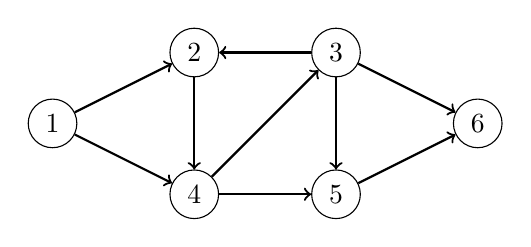
\begin{tikzpicture}[scale=0.9]
\node[draw, circle] (1) at (1,2) {$1$};
\node[draw, circle] (2) at (3,3) {$2$};
\node[draw, circle] (3) at (5,3) {$3$};
\node[draw, circle] (4) at (3,1) {$4$};
\node[draw, circle] (5) at (5,1) {$5$};
\node[draw, circle] (6) at (7,2) {$6$};
\path[draw,thick,->] (1) -- (2);
\path[draw,thick,->] (1) -- (4);
\path[draw,thick,->] (2) -- (4);
\path[draw,thick,->] (3) -- (2);
\path[draw,thick,->] (3) -- (5);
\path[draw,thick,->] (3) -- (6);
\path[draw,thick,->] (4) -- (3);
\path[draw,thick,->] (4) -- (5);
\path[draw,thick,->] (5) -- (6);
\end{tikzpicture}
\end{center}

Графтағы қырлары қиылыспайтын жолдардың максималды саны
2-ге тең. Біз $1 \rightarrow 2 \rightarrow 4 \rightarrow 3 \rightarrow 6$
және $1 \rightarrow 4 \rightarrow 5 \rightarrow 6$ жолдарын
таңдай аламыз:

\begin{center}
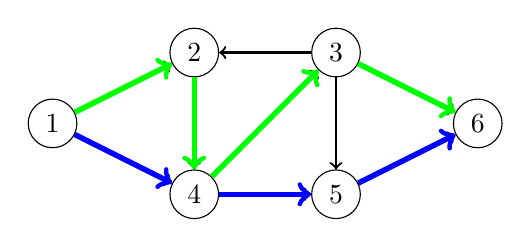
\begin{tikzpicture}[scale=0.9]
\node[draw, circle] (1) at (1,2) {$1$};
\node[draw, circle] (2) at (3,3) {$2$};
\node[draw, circle] (3) at (5,3) {$3$};
\node[draw, circle] (4) at (3,1) {$4$};
\node[draw, circle] (5) at (5,1) {$5$};
\node[draw, circle] (6) at (7,2) {$6$};
\path[draw,thick,->] (1) -- (2);
\path[draw,thick,->] (1) -- (4);
\path[draw,thick,->] (2) -- (4);
\path[draw,thick,->] (3) -- (2);
\path[draw,thick,->] (3) -- (5);
\path[draw,thick,->] (3) -- (6);
\path[draw,thick,->] (4) -- (3);
\path[draw,thick,->] (4) -- (5);
\path[draw,thick,->] (5) -- (6);

\path[draw=green,thick,->,line width=2pt] (1) -- (2);
\path[draw=green,thick,->,line width=2pt] (2) -- (4);
\path[draw=green,thick,->,line width=2pt] (4) -- (3);
\path[draw=green,thick,->,line width=2pt] (3) -- (6);

\path[draw=blue,thick,->,line width=2pt] (1) -- (4);
\path[draw=blue,thick,->,line width=2pt] (4) -- (5);
\path[draw=blue,thick,->,line width=2pt] (5) -- (6);
\end{tikzpicture}
\end{center}

Егер граф қырларының сыйымдылығын бір деп алсақ,
қырлары қиылыспайтын жолдардың максималды саны
максималды ағынға тең болады. Максималды ағын құрастырылғаннан кейін
бастаудан сағаға апаратын 
жолдарды ашкөз алгоритм арқылы қарастырып,
қырлары қиылыспайтын жолдарды таба аламыз.

\subsubsection{Төбелері қиылыспайтын жолдар}

Келесі есепте
бастаудан сағаға дейін \key{төбелері қиылыспайтын
жолдар}дың максималды санын есептеп көрейік. 
Есепте әр төбе бастау мен сағадан басқа 
жолда ең көбі бір рет кездеседі. 
Төбелері қиылыспайтын жолдардың саны
қырлары қиылыспайтын жолдар санынан 
аз болуы мүмкін. 

Мысалы, төмендегі графта төбелері қиылыспайтын 
жолдардың максималды саны -- 1:

\begin{center}
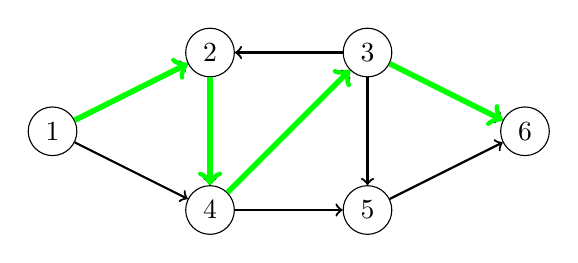
\begin{tikzpicture}
\node[draw, circle] (1) at (1,2) {$1$};
\node[draw, circle] (2) at (3,3) {$2$};
\node[draw, circle] (3) at (5,3) {$3$};
\node[draw, circle] (4) at (3,1) {$4$};
\node[draw, circle] (5) at (5,1) {$5$};
\node[draw, circle] (6) at (7,2) {$6$};
\path[draw,thick,->] (1) -- (2);
\path[draw,thick,->] (1) -- (4);
\path[draw,thick,->] (2) -- (4);
\path[draw,thick,->] (3) -- (2);
\path[draw,thick,->] (3) -- (5);
\path[draw,thick,->] (3) -- (6);
\path[draw,thick,->] (4) -- (3);
\path[draw,thick,->] (4) -- (5);
\path[draw,thick,->] (5) -- (6);

\path[draw=green,thick,->,line width=2pt] (1) -- (2);
\path[draw=green,thick,->,line width=2pt] (2) -- (4);
\path[draw=green,thick,->,line width=2pt] (4) -- (3);
\path[draw=green,thick,->,line width=2pt] (3) -- (6);
\end{tikzpicture}
\end{center}

Бұл есепті де максималды ағын есебіне келтірсек болады. 
Әр төбе жолда ең көбі бір рет бола алғандықтан
төбеден өтетін ағынды шектеуіміз қажет. Бұл үшін стандартты әдісті қолданып,
әр төбені екі төбеге бөлеміз. Бірінші төбе бастапқы төбеден кіріс қырларды қамтыса,
екінші төбе бастапқы төбеден шығыс қырларды қамтиды және бірінші төбеден
екінші төбеге жаңа қыр түседі. 

% We can reduce also this problem to the maximum flow problem.
% Since each node can appear in at most one path,
% we have to limit the flow that goes through the nodes.
% A standard method for this is to divide each node into
% two nodes such that the first node has the incoming edges
% of the original node, the second node has the outgoing
% edges of the original node, and
% there is a new edge from the first node
% to the second node.

Графымыз төмендегідей ретпен өзгереді:
\begin{center}
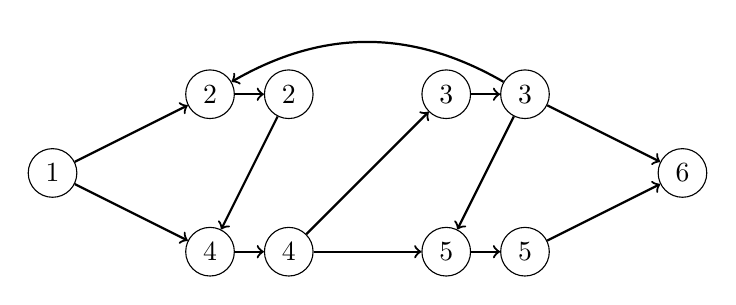
\begin{tikzpicture}
\node[draw, circle] (1) at (1,2) {$1$};

\node[draw, circle] (2a) at (3,3) {$2$};
\node[draw, circle] (3a) at (6,3) {$3$};
\node[draw, circle] (4a) at (3,1) {$4$};
\node[draw, circle] (5a) at (6,1) {$5$};

\node[draw, circle] (2b) at (4,3) {$2$};
\node[draw, circle] (3b) at (7,3) {$3$};
\node[draw, circle] (4b) at (4,1) {$4$};
\node[draw, circle] (5b) at (7,1) {$5$};

\node[draw, circle] (6) at (9,2) {$6$};

\path[draw,thick,->] (2a) -- (2b);
\path[draw,thick,->] (3a) -- (3b);
\path[draw,thick,->] (4a) -- (4b);
\path[draw,thick,->] (5a) -- (5b);

\path[draw,thick,->] (1) -- (2a);
\path[draw,thick,->] (1) -- (4a);
\path[draw,thick,->] (2b) -- (4a);
\path[draw,thick,->] (3b) edge [bend right=30] (2a);
\path[draw,thick,->] (3b) -- (5a);
\path[draw,thick,->] (3b) -- (6);
\path[draw,thick,->] (4b) -- (3a);
\path[draw,thick,->] (4b) -- (5a);
\path[draw,thick,->] (5b) -- (6);
\end{tikzpicture}
\end{center}

Графтағы максималды ағын:
\begin{center}
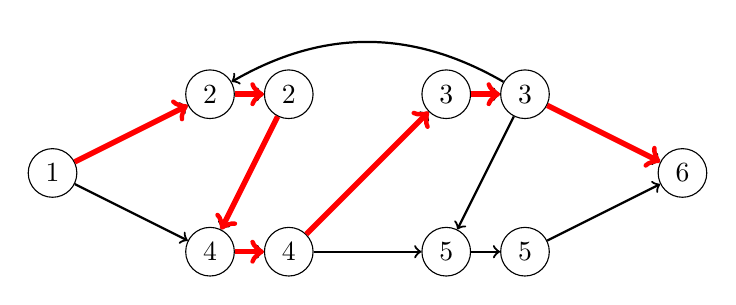
\begin{tikzpicture}
\node[draw, circle] (1) at (1,2) {$1$};

\node[draw, circle] (2a) at (3,3) {$2$};
\node[draw, circle] (3a) at (6,3) {$3$};
\node[draw, circle] (4a) at (3,1) {$4$};
\node[draw, circle] (5a) at (6,1) {$5$};

\node[draw, circle] (2b) at (4,3) {$2$};
\node[draw, circle] (3b) at (7,3) {$3$};
\node[draw, circle] (4b) at (4,1) {$4$};
\node[draw, circle] (5b) at (7,1) {$5$};

\node[draw, circle] (6) at (9,2) {$6$};

\path[draw,thick,->] (2a) -- (2b);
\path[draw,thick,->] (3a) -- (3b);
\path[draw,thick,->] (4a) -- (4b);
\path[draw,thick,->] (5a) -- (5b);

\path[draw,thick,->] (1) -- (2a);
\path[draw,thick,->] (1) -- (4a);
\path[draw,thick,->] (2b) -- (4a);
\path[draw,thick,->] (3b) edge [bend right=30] (2a);
\path[draw,thick,->] (3b) -- (5a);
\path[draw,thick,->] (3b) -- (6);
\path[draw,thick,->] (4b) -- (3a);
\path[draw,thick,->] (4b) -- (5a);
\path[draw,thick,->] (5b) -- (6);

\path[draw=red,thick,->,line width=2pt] (1) -- (2a);
\path[draw=red,thick,->,line width=2pt] (2a) -- (2b);
\path[draw=red,thick,->,line width=2pt] (2b) -- (4a);
\path[draw=red,thick,->,line width=2pt] (4a) -- (4b);
\path[draw=red,thick,->,line width=2pt] (4b) -- (3a);
\path[draw=red,thick,->,line width=2pt] (3a) -- (3b);
\path[draw=red,thick,->,line width=2pt] (3b) -- (6);
\end{tikzpicture}
\end{center}

Осылайша бастаудан сағаға дейінгі
төбелері қиылыспайтын жолдардың
максималды саны 1 болады.

\section{Максималды жұптасу}

\index{жұптасу}
\index{максималды жұптасу}

Максималды жұптасу есебінде тапсырма ретінде бағытталмаған графта
қырлар арқылы қосылып, әр төбе ең көбі бір жұпта болатын 
максималды төбелер жұптарының санын табу беріледі.

% The \key{maximum matching} problem asks to find
% a maximum-size set of node pairs in an undirected graph
% such that each pair is connected with an edge and
% each node belongs to at most one pair.

Жалпы графтарда максималды жұптасуды іздейтін 
полиномдық алгоритмдер бар\cite{edm65}, бірақ
ондай алгоритмдер күрделі және 
бағдарламау контесттерінде сирек кездеседі. 
Дегенмен екі ұялы графта максималды жұптасуды 
табу оңайырақ, өйткені біз оны максималды 
ағын есебіне келтіре аламыз. 

\subsubsection{Максималды жұптасуды іздеу}

Екі ұялы графтағы төбелерді қырлары сол топтан оң топқа бағытталатындай етіп,
әрдайым екі топқа бөле аламыз. Мысалы, төмендегі графтағы екі топ --  
$\{1,2,3,4\}$ және $\{5,6,7,8\}$.

\begin{center}
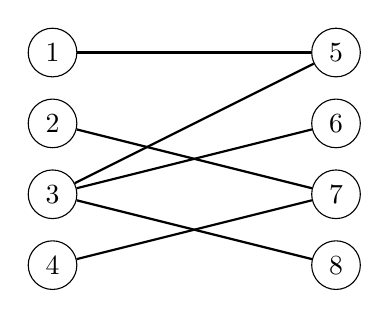
\begin{tikzpicture}[scale=0.60]
\node[draw, circle] (1) at (2,4.5) {1};
\node[draw, circle] (2) at (2,3) {2};
\node[draw, circle] (3) at (2,1.5) {3};
\node[draw, circle] (4) at (2,0) {4};
\node[draw, circle] (5) at (8,4.5) {5};
\node[draw, circle] (6) at (8,3) {6};
\node[draw, circle] (7) at (8,1.5) {7};
\node[draw, circle] (8) at (8,0) {8};

\path[draw,thick,-] (1) -- (5);
\path[draw,thick,-] (2) -- (7);
\path[draw,thick,-] (3) -- (5);
\path[draw,thick,-] (3) -- (6);
\path[draw,thick,-] (3) -- (8);
\path[draw,thick,-] (4) -- (7);
\end{tikzpicture}
\end{center}
Графтың максималды жұптасуының өлшемі -- 3:
\begin{center}
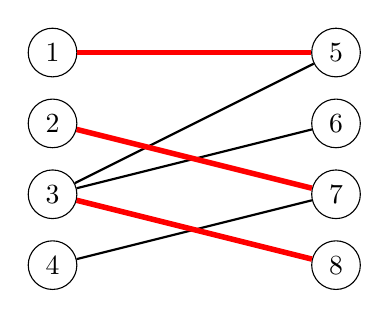
\begin{tikzpicture}[scale=0.60]
\node[draw, circle] (1) at (2,4.5) {1};
\node[draw, circle] (2) at (2,3) {2};
\node[draw, circle] (3) at (2,1.5) {3};
\node[draw, circle] (4) at (2,0) {4};
\node[draw, circle] (5) at (8,4.5) {5};
\node[draw, circle] (6) at (8,3) {6};
\node[draw, circle] (7) at (8,1.5) {7};
\node[draw, circle] (8) at (8,0) {8};

\path[draw,thick,-] (1) -- (5);
\path[draw,thick,-] (2) -- (7);
\path[draw,thick,-] (3) -- (5);
\path[draw,thick,-] (3) -- (6);
\path[draw,thick,-] (3) -- (8);
\path[draw,thick,-] (4) -- (7);

\path[draw=red,thick,-,line width=2pt] (1) -- (5);
\path[draw=red,thick,-,line width=2pt] (2) -- (7);
\path[draw=red,thick,-,line width=2pt] (3) -- (8);
\end{tikzpicture}
\end{center}

Максималды жұптасу есебін
бастау мен саға төбелерін қосу арқылы
максималды ағын есебіне келтіре аламыз.
Оған қоса, бастаудан сол жақ топтағы барлық төбелерге қырлар қосып,
сағаға оң жақ топтағы барлық төбелерден қырлар қосамыз.
Кейін осы графтағы максималды ағынның өлшемі берілген графтағы
максималды жұптасу өлшеміне тең болады. 

Мысалы, жаңа өзгерген графымыз төмендегідей болады:
\begin{center}
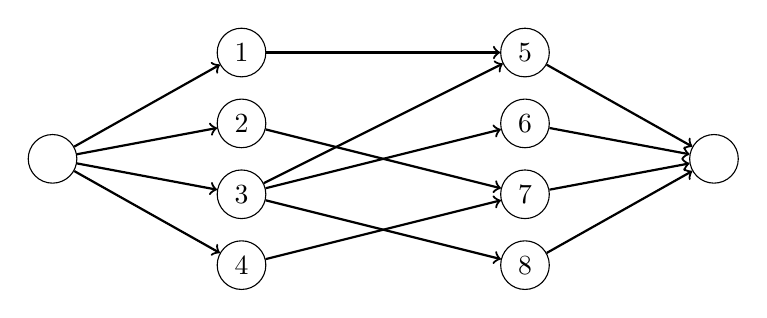
\begin{tikzpicture}[scale=0.60]
\node[draw, circle] (1) at (2,4.5) {1};
\node[draw, circle] (2) at (2,3) {2};
\node[draw, circle] (3) at (2,1.5) {3};
\node[draw, circle] (4) at (2,0) {4};
\node[draw, circle] (5) at (8,4.5) {5};
\node[draw, circle] (6) at (8,3) {6};
\node[draw, circle] (7) at (8,1.5) {7};
\node[draw, circle] (8) at (8,0) {8};

\node[draw, circle] (a) at (-2,2.25) {\phantom{0}};
\node[draw, circle] (b) at (12,2.25) {\phantom{0}};

\path[draw,thick,->] (1) -- (5);
\path[draw,thick,->] (2) -- (7);
\path[draw,thick,->] (3) -- (5);
\path[draw,thick,->] (3) -- (6);
\path[draw,thick,->] (3) -- (8);
\path[draw,thick,->] (4) -- (7);

\path[draw,thick,->] (a) -- (1);
\path[draw,thick,->] (a) -- (2);
\path[draw,thick,->] (a) -- (3);
\path[draw,thick,->] (a) -- (4);
\path[draw,thick,->] (5) -- (b);
\path[draw,thick,->] (6) -- (b);
\path[draw,thick,->] (7) -- (b);
\path[draw,thick,->] (8) -- (b);
\end{tikzpicture}
\end{center}

Графтың максималды ағыны келесідей болмақ:
\begin{center}
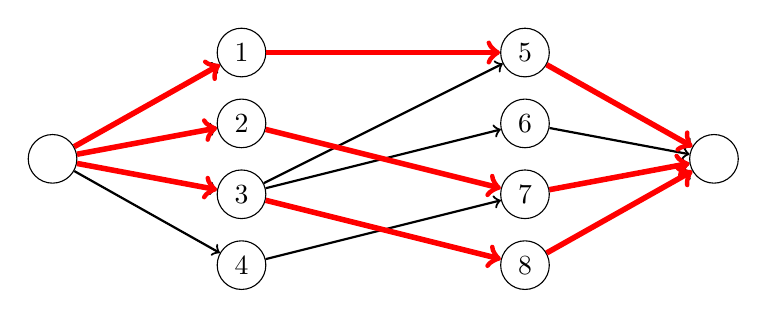
\begin{tikzpicture}[scale=0.60]
\node[draw, circle] (1) at (2,4.5) {1};
\node[draw, circle] (2) at (2,3) {2};
\node[draw, circle] (3) at (2,1.5) {3};
\node[draw, circle] (4) at (2,0) {4};
\node[draw, circle] (5) at (8,4.5) {5};
\node[draw, circle] (6) at (8,3) {6};
\node[draw, circle] (7) at (8,1.5) {7};
\node[draw, circle] (8) at (8,0) {8};

\node[draw, circle] (a) at (-2,2.25) {\phantom{0}};
\node[draw, circle] (b) at (12,2.25) {\phantom{0}};

\path[draw,thick,->] (3) -- (5);
\path[draw,thick,->] (3) -- (6);
\path[draw,thick,->] (4) -- (7);

\path[draw,thick,->] (a) -- (1);
\path[draw,thick,->] (a) -- (2);
\path[draw,thick,->] (a) -- (3);
\path[draw,thick,->] (a) -- (4);
\path[draw,thick,->] (5) -- (b);
\path[draw,thick,->] (6) -- (b);
\path[draw,thick,->] (7) -- (b);
\path[draw,thick,->] (8) -- (b);

\path[draw=red,thick,->,line width=2pt] (1) -- (5);
\path[draw=red,thick,->,line width=2pt] (2) -- (7);
\path[draw=red,thick,->,line width=2pt] (3) -- (8);

\path[draw=red,thick,->,line width=2pt] (a) -- (1);
\path[draw=red,thick,->,line width=2pt] (a) -- (2);
\path[draw=red,thick,->,line width=2pt] (a) -- (3);

\path[draw=red,thick,->,line width=2pt] (5) -- (b);
\path[draw=red,thick,->,line width=2pt] (7) -- (b);
\path[draw=red,thick,->,line width=2pt] (8) -- (b);

\end{tikzpicture}
\end{center}

\subsubsection{Хол теоремасы}

\index{Хол теоремасы}
\index{мінсіз жұптасу}

\key{Хол теоремасы} арқылы екі ұялы графта
барлық сол немесе оң жақ топтағы төбелерді қамтитын
жұптасудың бар-жоғын тексеруге болады. Егер 
сол мен оң жақ топтағы төбелердің сандары бірдей болса,
Хол теоремасы графтағы барлық төбелерді қамтитын
\key{мінсіз жұптасу} құрылысының 
мүмкін екендігін хабарлайды.

Мысалы, барлық сол жақ топтағы төбелерді қамтитын
жұптасуды тапқымыз келеді делік. 
$X$ деп кез келген сол жақ топтағы төбелер жиындысы 
және $f(X)$ деп олардың көршілерін белгілейік. 
Хол теоремасы бойынша әр $X$-ке $|X| \le |f(X)|$ шарты орындалған жағдайда ғана барлық сол жақ топтағы төбелерді
қамтитын жұптасу жүзеге асады. 
% eger tek eger degen qazaqwa iff degen fraza

Хол теоремасын граф мысалында қарайық.
Басында $X=\{1,3\}$ деп алсақ және
сәйкесінше $f(X)=\{5,6,8\}$ болса:

\begin{center}
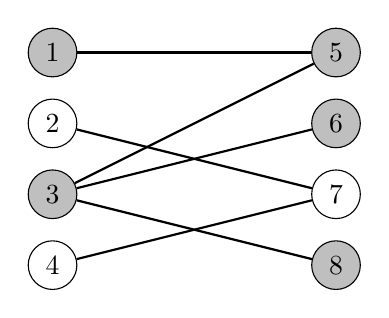
\begin{tikzpicture}[scale=0.60]
\node[draw, circle, fill=lightgray] (1) at (2,4.5) {1};
\node[draw, circle] (2) at (2,3) {2};
\node[draw, circle, fill=lightgray] (3) at (2,1.5) {3};
\node[draw, circle] (4) at (2,0) {4};
\node[draw, circle, fill=lightgray] (5) at (8,4.5) {5};
\node[draw, circle, fill=lightgray] (6) at (8,3) {6};
\node[draw, circle] (7) at (8,1.5) {7};
\node[draw, circle, fill=lightgray] (8) at (8,0) {8};

\path[draw,thick,-] (1) -- (5);
\path[draw,thick,-] (2) -- (7);
\path[draw,thick,-] (3) -- (5);
\path[draw,thick,-] (3) -- (6);
\path[draw,thick,-] (3) -- (8);
\path[draw,thick,-] (4) -- (7);
\end{tikzpicture}
\end{center}

Хол теоремасының шарты сақталды. Себебі 
$|X|=2$ және $|f(X)|=3$. Келесі 
$X=\{2,4\}$ деп алайық және 
сәйкесінше $f(X)=\{7\}$ болсын:

\begin{center}
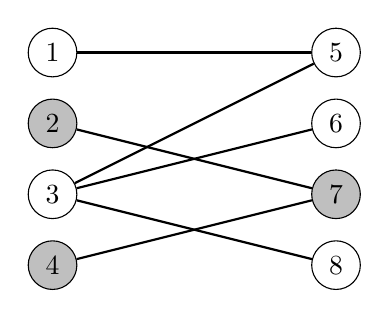
\begin{tikzpicture}[scale=0.60]
\node[draw, circle] (1) at (2,4.5) {1};
\node[draw, circle, fill=lightgray] (2) at (2,3) {2};
\node[draw, circle] (3) at (2,1.5) {3};
\node[draw, circle, fill=lightgray] (4) at (2,0) {4};
\node[draw, circle] (5) at (8,4.5) {5};
\node[draw, circle] (6) at (8,3) {6};
\node[draw, circle, fill=lightgray] (7) at (8,1.5) {7};
\node[draw, circle] (8) at (8,0) {8};

\path[draw,thick,-] (1) -- (5);
\path[draw,thick,-] (2) -- (7);
\path[draw,thick,-] (3) -- (5);
\path[draw,thick,-] (3) -- (6);
\path[draw,thick,-] (3) -- (8);
\path[draw,thick,-] (4) -- (7);
\end{tikzpicture}
\end{center}

Осы жағдайда $|X|=2$ және $|f(X)|=1$,
яғни Хол теоремасының шарты орындалмады.
Бұл граф үшін мінсіз жұптасуды құру мүмкін 
емес дегенді білдіреді. Тұжырым таңқаларлық емес, өйткені
осыған дейін де осы графтың максималды 
ағыны 4 емес, 3 екенін білген болатынбыз. 

Егер Хол теоремасының шарты орындалмаса,
$X$ жиыны ондай жұптасу \emph{неге} бола алмайтынына
түсіндірме береді. $X$-те $f(X)$-тен төбелер 
көп болғандықтан, $X$-тің барлық төбелеріне жұп 
табылмайды. Мысалы, жоғарыдағы графта 2-төбе мен 4-төбе
екеуі де 7-төбемен байланысуы керек, бірақ ол мүмкін емес. 

\subsubsection{Кёниг теоремасы}

\index{Кёниг теоремасы}
\index{төбелер бүркемесі}
\index{минималды төбелер бүркемесі}

Графтың \key{минималды төбелер бүркемесі} -- графтағы
қырлардың әр шетінің кем дегенде біреуі
жиында болатын
минималды төбелер жиыны.
Жалпы графтың минималды төбелер бүркемесін 
табу NP-қиын есептер қатарынан саналады. Бірақ егер граф екі ұялы болса,
\key{Кёниг теоремасы} минималды төбелер бүркемесінің өлшемі
максималды жұптасу өлшемімен тең деп тұжырымдайды.
Осылайша біз минималды төбелер бүркемесін максималды ағын
алгоритмі арқылы таба аламыз. 

% A \key{minimum node cover} of a graph
% is a minimum set of nodes such that each edge of the graph
% has at least one endpoint in the set.

Төмендегі максималды жұптасу өлшемі 3-ке тең
графты қарастырайық:
\begin{center}
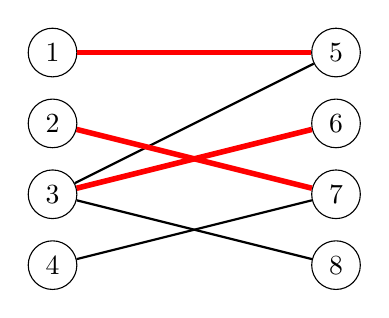
\begin{tikzpicture}[scale=0.60]
\node[draw, circle] (1) at (2,4.5) {1};
\node[draw, circle] (2) at (2,3) {2};
\node[draw, circle] (3) at (2,1.5) {3};
\node[draw, circle] (4) at (2,0) {4};
\node[draw, circle] (5) at (8,4.5) {5};
\node[draw, circle] (6) at (8,3) {6};
\node[draw, circle] (7) at (8,1.5) {7};
\node[draw, circle] (8) at (8,0) {8};

\path[draw,thick,-] (1) -- (5);
\path[draw,thick,-] (2) -- (7);
\path[draw,thick,-] (3) -- (5);
\path[draw,thick,-] (3) -- (6);
\path[draw,thick,-] (3) -- (8);
\path[draw,thick,-] (4) -- (7);

\path[draw=red,thick,-,line width=2pt] (1) -- (5);
\path[draw=red,thick,-,line width=2pt] (2) -- (7);
\path[draw=red,thick,-,line width=2pt] (3) -- (6);
\end{tikzpicture}
\end{center}
Кёниг теоремасы минималды төбелер бүркемесінің
өлшемі де 3 екенін айтады. 
Сондай бүркеме төмендегідей ретпен құрыстырылады:

\begin{center}
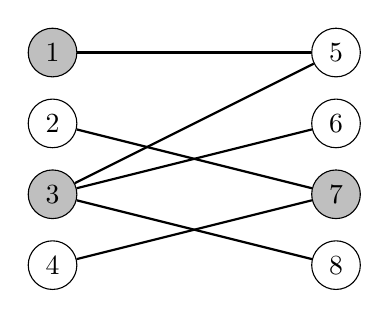
\begin{tikzpicture}[scale=0.60]
\node[draw, circle, fill=lightgray] (1) at (2,4.5) {1};
\node[draw, circle] (2) at (2,3) {2};
\node[draw, circle, fill=lightgray] (3) at (2,1.5) {3};
\node[draw, circle] (4) at (2,0) {4};
\node[draw, circle] (5) at (8,4.5) {5};
\node[draw, circle] (6) at (8,3) {6};
\node[draw, circle, fill=lightgray] (7) at (8,1.5) {7};
\node[draw, circle] (8) at (8,0) {8};

\path[draw,thick,-] (1) -- (5);
\path[draw,thick,-] (2) -- (7);
\path[draw,thick,-] (3) -- (5);
\path[draw,thick,-] (3) -- (6);
\path[draw,thick,-] (3) -- (8);
\path[draw,thick,-] (4) -- (7);
\end{tikzpicture}
\end{center}

\index{тәуелсіз жиын}
\index{максималды тәуелсіз жиын}

Минималды төбелер бүркемесіне \emph{кірмейтін}
төбелер \key{максималды тәуелсіз жиын}ды құрайды.
Бұл -- оған тиесілі екі төбенің ешқайсысы қырлармен байланыспайтын, төбелердің мүмкін болатын максималды жиыны. 
Қайталап өтейік, жалпы графтарда 
максималды тәуелсіз жиынды табу NP-қиын есеп саналады,
бірақ екі ұялы графтарда есепті Кёниг теоремасы
арқылы тиімдірек шешуге болады.
Мысалдағы графта максималды тәуелсіз жиын төмендегідей 
болады:

\begin{center}
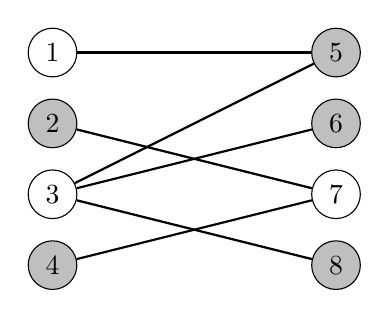
\begin{tikzpicture}[scale=0.60]
\node[draw, circle] (1) at (2,4.5) {1};
\node[draw, circle, fill=lightgray] (2) at (2,3) {2};
\node[draw, circle] (3) at (2,1.5) {3};
\node[draw, circle, fill=lightgray] (4) at (2,0) {4};
\node[draw, circle, fill=lightgray] (5) at (8,4.5) {5};
\node[draw, circle, fill=lightgray] (6) at (8,3) {6};
\node[draw, circle] (7) at (8,1.5) {7};
\node[draw, circle, fill=lightgray] (8) at (8,0) {8};

\path[draw,thick,-] (1) -- (5);
\path[draw,thick,-] (2) -- (7);
\path[draw,thick,-] (3) -- (5);
\path[draw,thick,-] (3) -- (6);
\path[draw,thick,-] (3) -- (8);
\path[draw,thick,-] (4) -- (7);
\end{tikzpicture}
\end{center}

\section{Жол бүркемелері}

\index{Жол бүркемесі}

\key{Жол бүркемесі} -- графтың әрбір төбесі кем дегенде 
бір жолға жататын жолдар жиынтығы. Бағытталған,
циклсіз графта минималды жол бүркеме есебін 
басқа графтағы максималды ағын табу есебіне келтіре 
аламыз.

\subsubsection{Төбелері қиылыспайтын жол бүркемесі}

\key{Төбелері қиылыспайтын жол бүркемесі}нде 
әр төбе тек бір жолға жатады.
Үлгі ретінде төмендегі графты қарастырайық:
\begin{center}
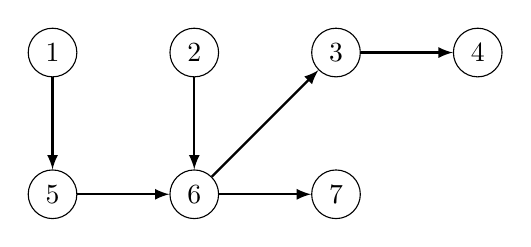
\begin{tikzpicture}[scale=0.9]
\node[draw, circle] (1) at (0,0) {1};
\node[draw, circle] (2) at (2,0) {2};
\node[draw, circle] (3) at (4,0) {3};
\node[draw, circle] (4) at (6,0) {4};
\node[draw, circle] (5) at (0,-2) {5};
\node[draw, circle] (6) at (2,-2) {6};
\node[draw, circle] (7) at (4,-2) {7};

\path[draw,thick,->,>=latex] (1) -- (5);
\path[draw,thick,->,>=latex] (2) -- (6);
\path[draw,thick,->,>=latex] (3) -- (4);
\path[draw,thick,->,>=latex] (5) -- (6);
\path[draw,thick,->,>=latex] (6) -- (3);
\path[draw,thick,->,>=latex] (6) -- (7);
\end{tikzpicture}
\end{center}

Графтағы минималды төбелері қиылыспайтын 
жол бүркемесі 3 жолдан тұрады.
Мысалы, төмендегі үш жолды таңдасақ болады:

\begin{center}
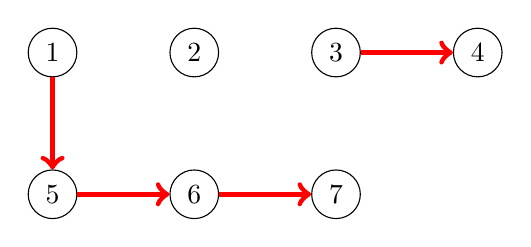
\begin{tikzpicture}[scale=0.9]
\node[draw, circle] (1) at (0,0) {1};
\node[draw, circle] (2) at (2,0) {2};
\node[draw, circle] (3) at (4,0) {3};
\node[draw, circle] (4) at (6,0) {4};
\node[draw, circle] (5) at (0,-2) {5};
\node[draw, circle] (6) at (2,-2) {6};
\node[draw, circle] (7) at (4,-2) {7};

\path[draw=red,thick,->,line width=2pt] (1) -- (5);
\path[draw=red,thick,->,line width=2pt] (5) -- (6);
\path[draw=red,thick,->,line width=2pt] (6) -- (7);
\path[draw=red,thick,->,line width=2pt] (3) -- (4);
\end{tikzpicture}
\end{center}

Жолдардың біреуі тек 2-төбеден тұратынына назар
аударыңыз, яғни жолда ешқандай қыр болмауы мүмкін.  

Минималды төбелері қиылыспайтын 
жол бүркемесін
берілген графтың әр төбесін оң және сол 
төбелермен бейнелейтін
\emph{жұптасу графын} құрастырып 
табуға болады. Егер бастапқы графта сол жақ төбеден оң жақ төбеге қарай қыр болса, жұптасу графында қыр сол жақ және оң жақ төбелердің арасынан өтеді. Оған қоса жұптасу графы бастау мен сағаны қамтиды.
Бастаудан барлық сол жақ төбелерге қырлар өтеді
және сағаға барлық оң жақ төбелерден қырлар өтеді. 


% We can find a minimum node-disjoint path cover
% by constructing a \emph{matching graph} where each node
% of the original graph is represented by
% two nodes: a left node and a right node.

Жаңа графтағы максималды жұптасу
берілген графтағы минималды төбелері қиылыспайтын 
жол бүркемесіне сәйкес болмақ. Мысалы, жоғарыдағы графтың жұптасу
графының максималды жұптасуының өлшемі 4-ке тең:

\begin{center}
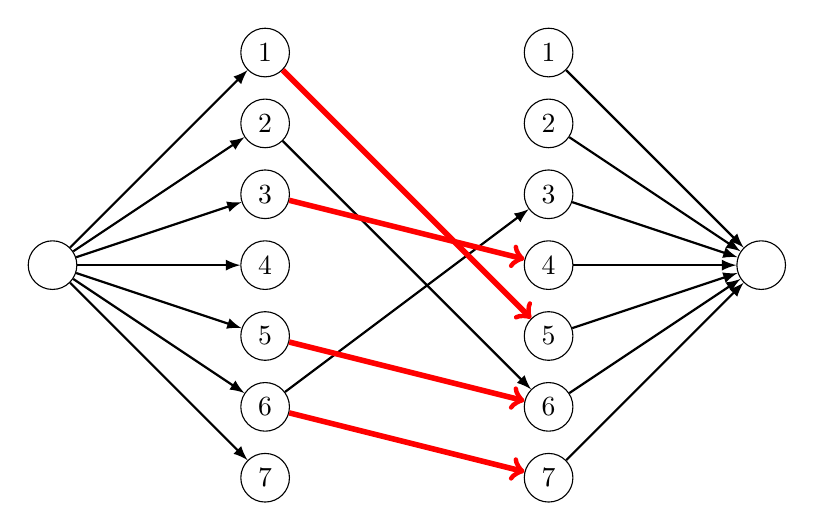
\begin{tikzpicture}[scale=0.9]
\node[draw, circle] (1a) at (0,6) {1};
\node[draw, circle] (2a) at (0,5) {2};
\node[draw, circle] (3a) at (0,4) {3};
\node[draw, circle] (4a) at (0,3) {4};
\node[draw, circle] (5a) at (0,2) {5};
\node[draw, circle] (6a) at (0,1) {6};
\node[draw, circle] (7a) at (0,0) {7};

\node[draw, circle] (1b) at (4,6) {1};
\node[draw, circle] (2b) at (4,5) {2};
\node[draw, circle] (3b) at (4,4) {3};
\node[draw, circle] (4b) at (4,3) {4};
\node[draw, circle] (5b) at (4,2) {5};
\node[draw, circle] (6b) at (4,1) {6};
\node[draw, circle] (7b) at (4,0) {7};

\node[draw, circle] (a) at (-3,3) {\phantom{0}};
\node[draw, circle] (b) at (7,3) {\phantom{0}};

%\path[draw,thick,->,>=latex] (1a) -- (5b);
\path[draw,thick,->,>=latex] (2a) -- (6b);
%\path[draw,thick,->,>=latex] (3a) -- (4b);
%\path[draw,thick,->,>=latex] (5a) -- (6b);
\path[draw,thick,->,>=latex] (6a) -- (3b);
%\path[draw,thick,->,>=latex] (6a) -- (7b);

\path[draw,thick,->,>=latex] (a) -- (1a);
\path[draw,thick,->,>=latex] (a) -- (2a);
\path[draw,thick,->,>=latex] (a) -- (3a);
\path[draw,thick,->,>=latex] (a) -- (4a);
\path[draw,thick,->,>=latex] (a) -- (5a);
\path[draw,thick,->,>=latex] (a) -- (6a);
\path[draw,thick,->,>=latex] (a) -- (7a);

\path[draw,thick,->,>=latex] (1b) -- (b);
\path[draw,thick,->,>=latex] (2b) -- (b);
\path[draw,thick,->,>=latex] (3b) -- (b);
\path[draw,thick,->,>=latex] (4b) -- (b);
\path[draw,thick,->,>=latex] (5b) -- (b);
\path[draw,thick,->,>=latex] (6b) -- (b);
\path[draw,thick,->,>=latex] (7b) -- (b);

\path[draw=red,thick,->,line width=2pt] (1a) -- (5b);
\path[draw=red,thick,->,line width=2pt] (5a) -- (6b);
\path[draw=red,thick,->,line width=2pt] (6a) -- (7b);
\path[draw=red,thick,->,line width=2pt] (3a) -- (4b);

\end{tikzpicture}
\end{center}

Жұптасу графындағы максималды жұптасудың әр қыры
берілген графтағы төбелері қиылыспайтын 
жол бүркемесінің қырларына сәйкес келеді.
Демек минималды төбелері қиылыспайтын 
жол бүркемесінің өлшемі $n-c$ болады,
мұндағы $n$ берілген графтағы төбелер саны болса,
$c$ максималды жұптасудың өлшемі болмақ.
\subsubsection{Жалпы жол бүркемесі}

\key{Жалпы жол бүркемесі} -- төбелер бірден көп
жолдарда жата алатын жол бүркемесі.
Минималды жалпы жол бүркемесі минималды
төбелері қиылыспайтын жол бүркемесінен 
кіші болуы мүмкін, өйткені төбе жолдарда бірнеше мәрте
қолданылуы мүмкін.  

Келесі графты қарастырайық:
\begin{center}
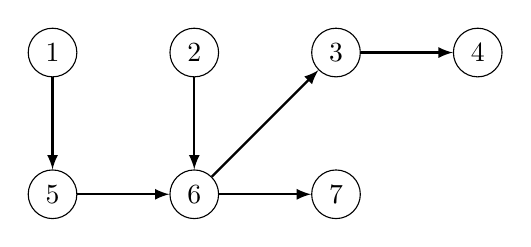
\begin{tikzpicture}[scale=0.9]
\node[draw, circle] (1) at (0,0) {1};
\node[draw, circle] (2) at (2,0) {2};
\node[draw, circle] (3) at (4,0) {3};
\node[draw, circle] (4) at (6,0) {4};
\node[draw, circle] (5) at (0,-2) {5};
\node[draw, circle] (6) at (2,-2) {6};
\node[draw, circle] (7) at (4,-2) {7};

\path[draw,thick,->,>=latex] (1) -- (5);
\path[draw,thick,->,>=latex] (2) -- (6);
\path[draw,thick,->,>=latex] (3) -- (4);
\path[draw,thick,->,>=latex] (5) -- (6);
\path[draw,thick,->,>=latex] (6) -- (3);
\path[draw,thick,->,>=latex] (6) -- (7);
\end{tikzpicture}
\end{center}

Графтың минималды жалпы жол бүркемесі екі 
жолдан тұрады. 
Мысалы, бірінші жол төмендегідей болуы мүмкін:
\begin{center}
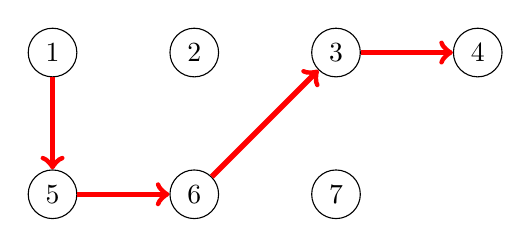
\begin{tikzpicture}[scale=0.9]
\node[draw, circle] (1) at (0,0) {1};
\node[draw, circle] (2) at (2,0) {2};
\node[draw, circle] (3) at (4,0) {3};
\node[draw, circle] (4) at (6,0) {4};
\node[draw, circle] (5) at (0,-2) {5};
\node[draw, circle] (6) at (2,-2) {6};
\node[draw, circle] (7) at (4,-2) {7};

\path[draw=red,thick,->,line width=2pt] (1) -- (5);
\path[draw=red,thick,->,line width=2pt] (5) -- (6);
\path[draw=red,thick,->,line width=2pt] (6) -- (3);
\path[draw=red,thick,->,line width=2pt] (3) -- (4);
\end{tikzpicture}
\end{center}
Ал екінші жол осындай болуы мүмкін:
\begin{center}
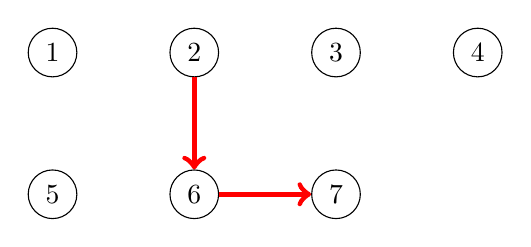
\begin{tikzpicture}[scale=0.9]
\node[draw, circle] (1) at (0,0) {1};
\node[draw, circle] (2) at (2,0) {2};
\node[draw, circle] (3) at (4,0) {3};
\node[draw, circle] (4) at (6,0) {4};
\node[draw, circle] (5) at (0,-2) {5};
\node[draw, circle] (6) at (2,-2) {6};
\node[draw, circle] (7) at (4,-2) {7};

\path[draw=red,thick,->,line width=2pt] (2) -- (6);
\path[draw=red,thick,->,line width=2pt] (6) -- (7);
\end{tikzpicture}
\end{center}

Минималды жалпы жол бүркемесін
төбелері қиылыспайтын минималды жол бүркемесі
сияқты табуға болады. Ол үшін
бастапқы графта $a$-дан $b$-ға (бәлкім бірнеше төбелер арқылы өтетін) жол болған жағдайда $a \rightarrow b$ қыры болатындай етіп, жұптасқан графқа тағы бірнеше қырлар қоссақ жеткілікі.

Жоғарыдағы графтың жұптасу графы төмендегідей болады:
\begin{center}
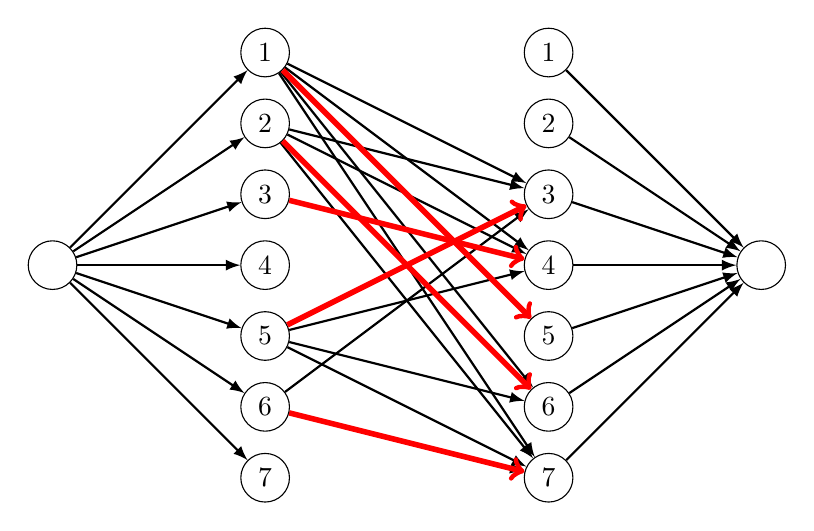
\begin{tikzpicture}[scale=0.9]
\node[draw, circle] (1a) at (0,6) {1};
\node[draw, circle] (2a) at (0,5) {2};
\node[draw, circle] (3a) at (0,4) {3};
\node[draw, circle] (4a) at (0,3) {4};
\node[draw, circle] (5a) at (0,2) {5};
\node[draw, circle] (6a) at (0,1) {6};
\node[draw, circle] (7a) at (0,0) {7};

\node[draw, circle] (1b) at (4,6) {1};
\node[draw, circle] (2b) at (4,5) {2};
\node[draw, circle] (3b) at (4,4) {3};
\node[draw, circle] (4b) at (4,3) {4};
\node[draw, circle] (5b) at (4,2) {5};
\node[draw, circle] (6b) at (4,1) {6};
\node[draw, circle] (7b) at (4,0) {7};

\node[draw, circle] (a) at (-3,3) {\phantom{0}};
\node[draw, circle] (b) at (7,3) {\phantom{0}};


%\path[draw,thick,->,>=latex] (1a) -- (5b);
\path[draw,thick,->,>=latex] (1a) -- (6b);
\path[draw,thick,->,>=latex] (1a) -- (7b);
\path[draw,thick,->,>=latex] (1a) -- (3b);
\path[draw,thick,->,>=latex] (1a) -- (4b);
\path[draw,thick,->,>=latex] (5a) -- (6b);
\path[draw,thick,->,>=latex] (5a) -- (7b);
%\path[draw,thick,->,>=latex] (5a) -- (3b);
\path[draw,thick,->,>=latex] (5a) -- (4b);
\path[draw,thick,->,>=latex] (6a) -- (7b);
%\path[draw,thick,->,>=latex] (6a) -- (7b);
\path[draw,thick,->,>=latex] (6a) -- (3b);
%\path[draw,thick,->,>=latex] (3a) -- (4b);
%\path[draw,thick,->,>=latex] (2a) -- (6b);
\path[draw,thick,->,>=latex] (2a) -- (7b);
\path[draw,thick,->,>=latex] (2a) -- (3b);
\path[draw,thick,->,>=latex] (2a) -- (4b);


\path[draw,thick,->,>=latex] (a) -- (1a);
\path[draw,thick,->,>=latex] (a) -- (2a);
\path[draw,thick,->,>=latex] (a) -- (3a);
\path[draw,thick,->,>=latex] (a) -- (4a);
\path[draw,thick,->,>=latex] (a) -- (5a);
\path[draw,thick,->,>=latex] (a) -- (6a);
\path[draw,thick,->,>=latex] (a) -- (7a);

\path[draw,thick,->,>=latex] (1b) -- (b);
\path[draw,thick,->,>=latex] (2b) -- (b);
\path[draw,thick,->,>=latex] (3b) -- (b);
\path[draw,thick,->,>=latex] (4b) -- (b);
\path[draw,thick,->,>=latex] (5b) -- (b);
\path[draw,thick,->,>=latex] (6b) -- (b);
\path[draw,thick,->,>=latex] (7b) -- (b);

\path[draw=red,thick,->,line width=2pt] (1a) -- (5b);
\path[draw=red,thick,->,line width=2pt] (5a) -- (3b);
\path[draw=red,thick,->,line width=2pt] (3a) -- (4b);
\path[draw=red,thick,->,line width=2pt] (2a) -- (6b);
\path[draw=red,thick,->,line width=2pt] (6a) -- (7b);


% \path[draw=red,thick,->,line width=2pt] (1a) -- (6b);
% \path[draw=red,thick,->,line width=2pt] (1a) -- (7b);
% \path[draw=red,thick,->,line width=2pt] (1a) -- (3b);
% \path[draw=red,thick,->,line width=2pt] (1a) -- (4b);
% \path[draw=red,thick,->,line width=2pt] (5a) -- (6b);
% \path[draw=red,thick,->,line width=2pt] (5a) -- (7b);
% \path[draw=red,thick,->,line width=2pt] (5a) -- (3b);
% \path[draw=red,thick,->,line width=2pt] (5a) -- (4b);
% \path[draw=red,thick,->,line width=2pt] (6a) -- (7b);
% \path[draw=red,thick,->,line width=2pt] (6a) -- (7b);
% \path[draw=red,thick,->,line width=2pt] (6a) -- (3b);
% \path[draw=red,thick,->,line width=2pt] (3a) -- (4b);
% \path[draw=red,thick,->,line width=2pt] (2a) -- (6b);
% \path[draw=red,thick,->,line width=2pt] (2a) -- (7b);
% \path[draw=red,thick,->,line width=2pt] (2a) -- (3b);
% \path[draw=red,thick,->,line width=2pt] (2a) -- (4b);

\end{tikzpicture}
\end{center}

\subsubsection{Дилуорс теоремасы}

\index{Дилуорс теоремасы}
\index{антитізбек}

\key{Антитізбек} -- бір төбеден екінші төбеге 
қырлар арқылы жол болмайтын төбелер жиындысы.
\key{Дилуорс теоремасы} бағытталған циклсіз графтың
минималды жалпы жол бүркемесінің өлшемі
максималды антитізбектің өлшеміне сәйкес деп мәлімдейді.

% An \key{antichain} is a set of nodes of a graph
% such that there is no path
% from any node to another node
% using the edges of the graph.

Мысалы төмендегі графта 3-төбе мен 7-төбе 
антитізбекті құрайды:

\begin{center}
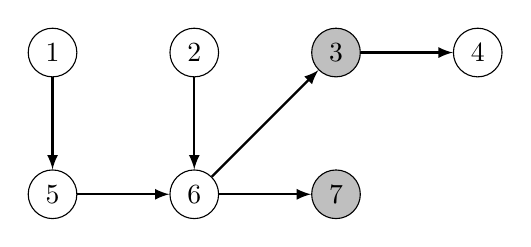
\begin{tikzpicture}[scale=0.9]
\node[draw, circle] (1) at (0,0) {1};
\node[draw, circle] (2) at (2,0) {2};
\node[draw, circle, fill=lightgray] (3) at (4,0) {3};
\node[draw, circle] (4) at (6,0) {4};
\node[draw, circle] (5) at (0,-2) {5};
\node[draw, circle] (6) at (2,-2) {6};
\node[draw, circle, fill=lightgray] (7) at (4,-2) {7};

\path[draw,thick,->,>=latex] (1) -- (5);
\path[draw,thick,->,>=latex] (2) -- (6);
\path[draw,thick,->,>=latex] (3) -- (4);
\path[draw,thick,->,>=latex] (5) -- (6);
\path[draw,thick,->,>=latex] (6) -- (3);
\path[draw,thick,->,>=latex] (6) -- (7);
\end{tikzpicture}
\end{center}

3 төбеден тұратын антитізбек
мүлдем құрастырылмайтын болғандықтан, мысалдығы тізбек максималды антитізбекке жатады. Осы графтың 
минималды жалпы жол бүркемесінің өлшемі 2 жолдан тұратынын осыған 
білген едік.
